\documentclass{article}
\usepackage[utf8]{inputenc}
\usepackage{titling}
\usepackage{graphicx}
\usepackage{grffile}
\usepackage{verbatim}
\usepackage{geometry}
 \geometry{
 a4paper,
 total={170mm,257mm},
 left=20mm,
 top=20mm,
 }

\setlength{\droptitle}{-7 em} 

\begin{document}

\title{ET4394: Wireshark Assignment}

\author{Saumil Sachdeva (4740998) and Niket Agrawal (4719514) | Group WN3
}
\date{\today}

\maketitle

\section{Introduction}

Through this project, we aim to acquire a better understanding of some of the commonly used WiFi parameters by analyzing the data captured in different environments and relating the findings with technical reasoning in the literature. 
Following parameters are analyzed:
\begin{enumerate}
    \item Wifi channels used- Which channel are mostly used and how it relates to the type of environment
    \item Channel size (whether channel bonding is used or not)
    \item PHY distribution
    \item Distribution of operating Frequency of the Access Points
\end{enumerate}


\section{Technical details about the parameters}

\begin{itemize}
    \item There are typically two frequency bands used for Wi-Fi technology, 2.4GHz and 5GHz.
    \begin{itemize}
        \item 2.4GHz band comprises of 11 channels each 20MHz wide and the entire band is 80MHz wide. Channels 1, 6 and 11 are the only non overlapping channels in this band. The 2.4GHz band offers a good range but is prone to congestion because of the presence of several overlapping channels.
        \item 5GHz band has 23 non overlapping channels each 20MHz wide which offers the opportunity to perform channel bonding by combining multiple 20MHz channels to form one channel of larger width. This provides improved speed and bandwidth to the user.
    \end{itemize}
    \item IEEE 802.11 WLAN standards:
    \begin{itemize}
        \item 802.11ac PHY type uses a 5GHz band. It achieves high speed and throughput by performing channel bonding and offering channel widths of 40MHz, 80 MHz or even 160MHz.
        \item 802.11n is a high throughput standard, which operates on 2.4GHz/5GHz and offers channel bonding feature for only 40MHz.
        \item Backwards Compatibility: 802.11ac is backward compatible with the previous standards so an ac type router can transmit packets with PHY type 802.11n and also 802.11a/b/g which are predecessors of 802.11n. 802.11n is backward compatible with 802.11a/b/g.
    \end{itemize}
\end{itemize}

\section{Experimental setup}

Since we are only interested in capturing 802.11 management and control packets or packets with only the RadioTap header information (these packets contain information about channel, frequency, channel width, etc), we put the network adapter on our PC in monitor mode and then passively listen on these packets. 
\begin{enumerate}
    \item Filtering for packet type
    \begin{itemize}
        \item Out of the packets that we receive, only beacon frames are of importance as these frames contain complete information about the network like the operating frequency, the channel it is using, PHY type, etc. These frames are transmitted periodically by the access point to announce its presence.
        \item Apart from beacons, other packets received are probe response packets sent by the access point in response to the probe request packets sent by the client (us) to acquire information from an access point. These packets contain the same information about the AP as the beacons so collecting and analyzing only the beacon frames is sufficient for the purpose of our project.
    \end{itemize}
    \item Choosing the capture environment
    \begin{itemize}
        \item Packet capture was done in three different environments with the motivation of collecting a data set which would cover multiple scenarios. Data was captured at a public place with several access points (dense environment), an academic environment (High quality WiFi infrastructure with multiple access points) and a dormitory residence (sparse environment with several access points)
    \end{itemize}
    \item Tools and scripts for packet capture
    \begin{itemize}
        \item TShark was used to capture and filter the packets for the desired information and converted to a JSON file format. The JSON file was then parsed using a python script to store all the information in an organized way in multiple dictionaries which were further used to generate plots representing the trends observed.
    \end{itemize}
    
\end{enumerate}

\section{Observations}

Packets captured in three different environments were analyzed after generating the plots for the parameters they used.

\subsection{De Hoven passage}
Packets were captured inside the Dehoven pasage shopping complex and the Albert Heijn in its vicinity on a weekend with a decent crowd. This data capture represents a dense environment with multiple access points. 

\begin{itemize}

    \item We observe from the plots in figure \ref{Fig. 1} that most of the routers were of PHY 'n' type operating at 2.4GHz which are capable of channel bonding for a channel width up to 40MHz. Being a free internet service in a public domain, very high throughput infrastructure and service is generally not expected, which is evident from the presence of considerably less number of AC type routers and 80MHz channel width in the plots and also by the presence of routers having the old WiFi standard PHY type of 802.11 b/g/a. In crowded areas with a lot of frequency noise and interference, a single 20MHz channel will be more stable. 40MHz channel width allows for greater speed and faster transfer rates but it doesn't perform as well in crowded areas.
    
     \item Since it's a dense environment and almost everyone is operating at 2.4GHz, contention for channel is an issue, so the access points try to use the non overlapping channels as much as possible, which is seen in the plots as well, channel 1, 6 and 11 being the mostly used channels. 
    
    \item Since the 802.11n PHY type is backward compatible with 802.11a/b/g, we notice that most of the messages transmitted are actually sent on phy '802.11 b' at 20MHz rather than '802.11 n'. The reason being that, 802.11 b is low cost and offers a good signal range, but the data rate is slow. Above features are quite common in a WiFi internet service provided in a public domain.
    
    
\end{itemize}

\begin{figure}[h]
      	\centering
     	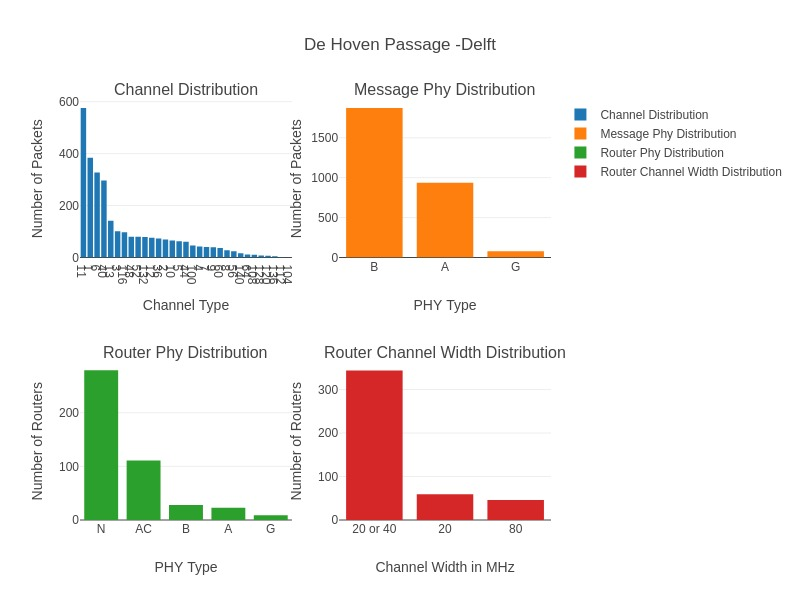
\includegraphics[scale=0.55]{De Hoven Passage -Delft.jpeg}
      	\caption{Distribution for Packets captured at Dehoven passage Delft}
      	\label{Fig. 1}
\end{figure}




\subsection{Dormitory in Delft}
Packets were captured in a dormitory in Delft with single occupancy rooms, almost each room has its own access point, which represents a sparse environment with multiple access points. The analysis is shown using the plots generated in figure \ref{Fig. 2}

\begin{itemize}
    \item A clear majority of routers were of 802.11n PHY type operating at 2.4GHz capable of channel bonding of up to 40MHz. 
    \item Most popular channels used were 6, 11 and 1 which are the only non overlapping channels in the 2.4GHz band. This is evident from the fact that since most of the routers operating in the 2.4GHz band would create a congestion, so using the non overlapping channels is the best choice. 
    \item Most messages are sent on 802.11b PHY type at 20MHz channel width rather than n because of backward compatibility as per the Message PHY Distribution plot in figure\ref{Fig. 2}
    \item Because there is a heavy contention for the channels in the 2.4GHz band, using a 5GHz band can offer better bandwidth and data rates. 5GHz also offers channel bonding capability with possibility to use 40MHz, 80 MHz and even 160MHz channel width. Even though 5GHz band is not good when it comes to range and penetrating obstacles, but because in this case there will be only very few people broadcasting at this frequency it will not create any congestion. Range is also not an issue because there is one router per room.
    
\end{itemize}


\begin{figure}[h]
      	\centering
     	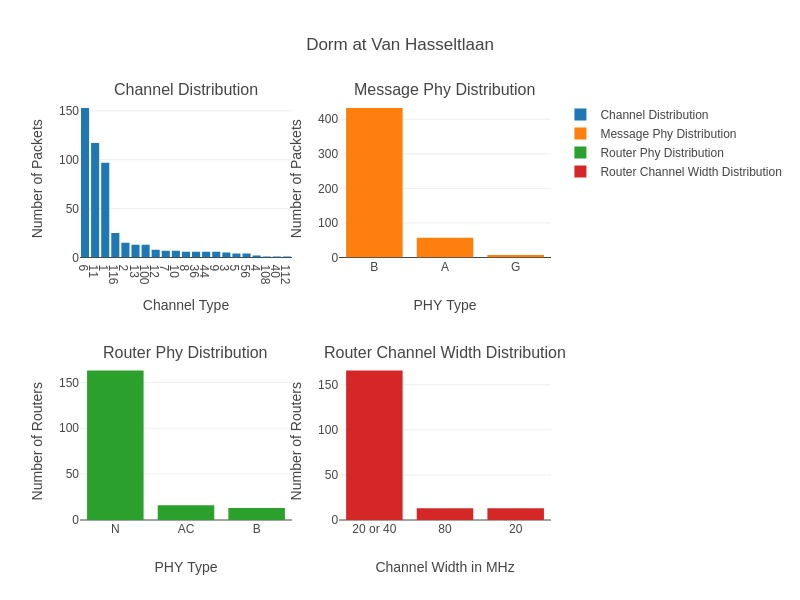
\includegraphics[scale=0.55]{Dorm at Van Hasseltlaan.jpeg}
      	\caption{Distribution for Packets captured in a dorm in Delft}
      	\label{Fig. 2}
\end{figure}

\subsection{Library at TU Delft}
Packets were capture inside the library at TU Delft. It represents a dense environment with multiple access points in an academic setting. The analysis is shown using the plots in figure \ref{Fig. 3}
\begin{itemize}
    \item An academic environment such as university campus or library generally provides a good infrastructure for WiFi internet. This can be deduced from the plot - Router PHY Distribution in figure \ref{Fig. 3}. Majority of the routers are of 802.11ac PHY type.
    
    \item Since the library at TU Delft is a dense environment with a significant number of students sitting with their laptops and accessing the network at the same time, channel bonding is not that common. A channel width of 80MHz or 160MHz will congest the local area and since many clients are accessing the network together in the library, this will affect everyone badly.
    
    \item Apart from channel '1', channel distribution is quite uniform here as compared to the previous two cases due to the majority of the routers which operate on the 5GHz band. Since 5GHz band offers 23 non overlapping channels, the contention for a specific channel is not present. 
    
    \item Most messages are sent on 802.11a PHY type unlike 801.11b in the case of Dehoven passage discussed earlier. This is because 802.11a provides faster data rate and prevents signal interference from other devices. The cost is more than 802.11b standard so it is more likely to be seen in an environment which possess better infrastructure like university campus.
\end{itemize}

\begin{figure}[h]
      	\centering
     	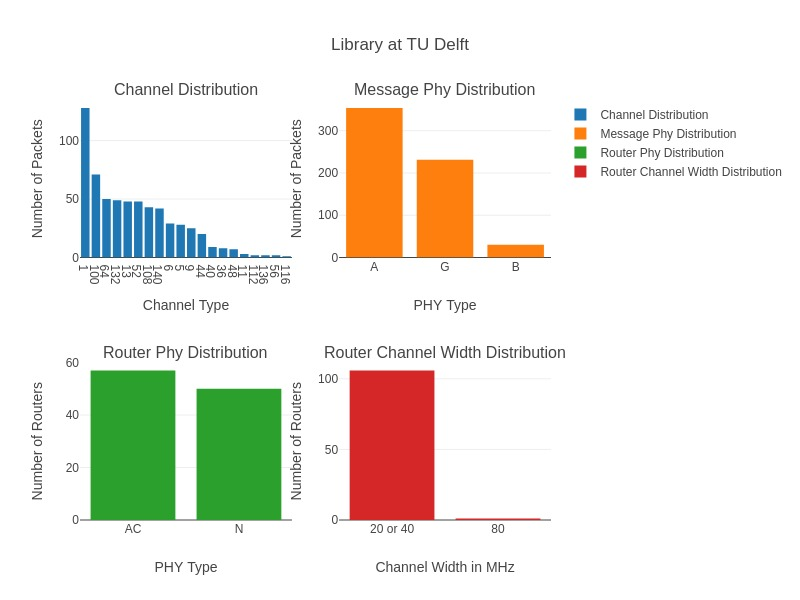
\includegraphics[scale=0.55]{Library at TU Delft.jpeg}
      	\caption{Distribution for Packets captured in library in TU Delft}
      	\label{Fig. 3}
\end{figure}

\section{Conclusion}

Through this project we were able to observe, reason and understand the technical aspects related to the WiFi usage in different environments as governed by various parameters and standards like channel, frequency, PHY, channel width, etc. Working on this project was an immense learning experience, right from getting to know how to passively capture network traffic, use the software tools and scripts for filtering, parsing, analyzing the data and to be able to relate the experimental observations with the technical aspects. 

\end{document}

